\chapter{Implementación de datos estructurados}
\label{chap:4}
En este capítulo, finalmente, nos toca hablar del primero de los dos sistemas implementados en este trabajo.
El sistema en cuestión implementa, con algunas limitaciones que mencionaremos, el modelo de Popescu descripto en \cite{QADB1} y \cite{QADB2} y reseñados por nosotros en \ref{subsec:closed-domain}.

Nuestro código está accesible públicamente en la siguiente dirección: \url{http://github.com/julian3833/popescu-world}. Allí pueden encontrarse, además del código en sí mismo, los procedimientos de instalación, ejemplos de ejecución y una lista con los principales puntos técnicos que pueden mejorarse (ver, también, \allref{subsec:popescu-cierre}).

Testeamos este sistema sobre la base de datos World, en inglés, ofrecida por MySQL\footnote{Ver \url{http://dev.mysql.com/doc/world-setup/en/index.html} y \url{http://dev.mysql.com/doc/index-other.html}} que consta de información geográfica básica sobre países, ciudades e idiomas.

Cabe mencionar que el scope original de este sistema era ser bilingüe y ejecutarse sobre una base de datos sobre universidades, empresas e investigación nacional del ámbito de la informática. Lamentablemente, por una cuestión de tiempos y de errores a la hora de estimar esfuerzos, no pudimos completar este plan original.

La estructura del capítulo es como sigue: En \ref{sec:popescu-db} pasamos revista de la base de datos que utilizamos para implementar el sistema y en \ref{sec:popescu-implementacion} discutimos la implementación. \ref{subsec:popescu-codigo} se divide, a su vez, en \ref{subsec:popescu-ejemplos}, donde discutimos la implementación en sí misma, 4.2.2, donde mostramos y comentamos algunos ejemplos de ejecuciones y \ref{subsec:popescu-cierre} donde analizamos los alcances, los límites y el trabajo futuro.


\section{Base de datos}
\label{sec:popescu-db}

La base de datos World consta de 3 tablas: Country, City y CountryLanguage (ver Figura \ref{fig:world-db}).

\begin{figure}
  \centering
    %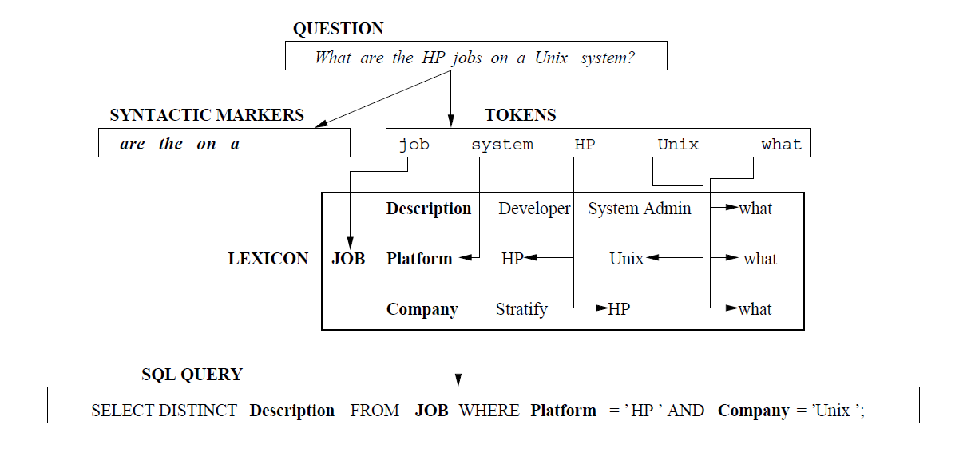
\includegraphics[scale=1.0]{graficos/popescu-example}
    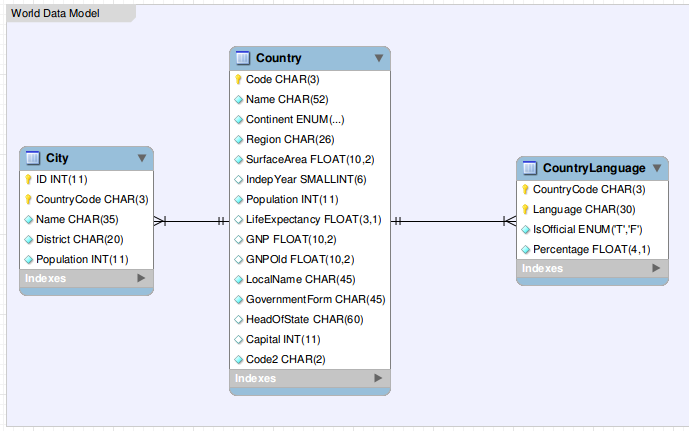
\includegraphics[width=12.823cm,height=8.004cm]{graficos/fuentes/world-db.png}
  \caption{Modelo entidad relación de la base de datos World original}
  \label{fig:world-db}
\end{figure}

La tabla Country tiene información básica acerca de varios países del mundo. La tabla City tiene información sobre las mayores ciudades del mundo y, finalmente, la tabla CountryLanguage tiene información sobre los idiomas hablados en cada país.

Hay una relación de uno a muchos entre Country y CountryLanguage: cada país puede tener más de un idioma y, además, hay una relación de uno a muchos entre Country y City: cada país puede tener más de una ciudad.

\medskip
Las definiciones de las relaciones originales son:
\begin{itemize}
\item Country(Code, Name, Continent, Region, SurfaceArea, IndepYear, Population, LifeExpectancy, GNP, GNPOld, LocalName, GovernmentForm, HeadOfState, Capital, Code2)
\item City(ID, ContryCode, Name, District, Population)
\item CountryLanguage(CountryCode, Language, IsOfficial, Percentage)
\end{itemize}

Para nuestro proyecto, renombramos algunos de los elementos:
\begin{itemize}
\item La relación CountryLanguage fue renombrada a Language
\item El atributo Language de la relación CountryLanguage fue renombrado a Name
\item El atributo IndepYear de la relación Country fue renombrado a IndependenceYear
\end{itemize}

%TODO: falta mencionar un cambio importante (reemplazo de los ids por los valores en una columna que no recuerdo)

En las tablas \ref{tab:country-data}, \ref{tab:country-data-2}, \ref{table:countrylanguage-data} y \ref{table:city-data} pueden verse algunas filas de ejemplo de cada una de las tablas y, en la tabla W, el total de filas de cada una.

%TODO: agregar que no soportamos IsOfficial a limites

%
% Data: countrylanguage
%
 \begin{longtable}{|l|l|l|l|}
 \hline \endhead \hline \endfoot \hline
 \caption{Algunas filas de la tabla CountryLanguage} \label{table:countrylanguage-data} \\\hline \multicolumn{1}{|c|}{\textbf{CountryCode}} & \multicolumn{1}{|c|}{\textbf{Language}} & \multicolumn{1}{|c|}{\textbf{IsOfficial}} & \multicolumn{1}{|c|}{\textbf{Percentage}} \\ \hline \hline  \endfirsthead
\caption{Content of table countrylanguage (continued)} \\ \hline \multicolumn{1}{|c|}{\textbf{CountryCode}} & \multicolumn{1}{|c|}{\textbf{Language}} & \multicolumn{1}{|c|}{\textbf{IsOfficial}} & \multicolumn{1}{|c|}{\textbf{Percentage}} \\ \hline \hline \endhead \endfoot
ABW & Dutch & T & 5.3 \\ \hline
ABW & English & F & 9.5 \\ \hline
ABW & Papiamento & F & 76.7 \\ \hline
ABW & Spanish & F & 7.4 \\ \hline
AFG & Balochi & F & 0.9 \\ \hline
AFG & Dari & T & 32.1 \\ \hline
AFG & Pashto & T & 52.4 \\ \hline
AFG & Turkmenian & F & 1.9 \\ \hline
AFG & Uzbek & F & 8.8 \\ \hline
AGO & Ambo & F & 2.4 \\ \hline
AGO & Chokwe & F & 4.2 \\ \hline
AGO & Kongo & F & 13.2 \\ \hline
AGO & Luchazi & F & 2.4 \\ \hline
 \end{longtable}

\clearpage % Las tablas se ubican mal, no se xq
%
% Data: city
%
  \begin{longtable}{|l|l|l|l|l|}
 \hline \endhead \hline \endfoot \hline
 \caption{Algunas filas de la relación City} \label{table:city-data} \\\hline \multicolumn{1}{|c|}{\textbf{ID}} & \multicolumn{1}{|c|}{\textbf{Name}} & \multicolumn{1}{|c|}{\textbf{CountryCode}} & \multicolumn{1}{|c|}{\textbf{District}} & \multicolumn{1}{|c|}{\textbf{Population}} \\ \hline \hline  \endfirsthead
\caption{Algunas filas de la tabla city} \\ \hline \multicolumn{1}{|c|}{\textbf{ID}} & \multicolumn{1}{|c|}{\textbf{Name}} & \multicolumn{1}{|c|}{\textbf{CountryCode}} & \multicolumn{1}{|c|}{\textbf{District}} & \multicolumn{1}{|c|}{\textbf{Population}} \\ \hline \hline \endhead \endfoot
129 & Oranjestad & ABW & – & 29034 \\ \hline
1 & Kabul & AFG & Kabol & 1780000 \\ \hline
56 & Luanda & AGO & Luanda & 2022000 \\ \hline
61 & South Hill & AIA & – & 961 \\ \hline
34 & Tirana & ALB & Tirana & 270000 \\ \hline
55 & Andorra la Vella & AND & Andorra la Vella & 21189 \\ \hline
33 & Willemstad & ANT & Curaçao & 2345 \\ \hline
64 & Dubai & ARE & Dubai & 669181 \\ \hline
69 & Buenos Aires & ARG & Distrito Federal & 2982146 \\ \hline
126 & Yerevan & ARM & Yerevan & 1248700 \\ \hline
53 & Tafuna & ASM & Tutuila & 5200 \\ \hline
63 & Saint John's & ATG & St John & 24000 \\ \hline
130 & Sydney & AUS & New South Wales & 3276207 \\ \hline
 \end{longtable}

\bigskip
%
% Data: country
%
\begin{footnotesize}
 \begin{longtable}{|l|l|l|l|l|l|}
 \hline \endhead \hline \endfoot \hline
 \caption{Algunas filas de la tabla Country} \label{tab:country-data} \\\hline \multicolumn{1}{|c|}{\textbf{Code}} & \multicolumn{1}{|c|}{\textbf{Name}} & \multicolumn{1}{|c|}{\textbf{Continent}} & \multicolumn{1}{|c|}{\textbf{Region}} & \multicolumn{1}{|c|}{\textbf{SurfaceArea}} & \multicolumn{1}{|c|}{\textbf{IndepYear}} \\ \hline \hline  \endfirsthead
\caption{Algunas filas de la tabla Country} \\ \hline \multicolumn{1}{|c|}{\textbf{Code}} & \multicolumn{1}{|c|}{\textbf{Name}} & \multicolumn{1}{|c|}{\textbf{Continent}} & \multicolumn{1}{|c|}{\textbf{Region}} & \multicolumn{1}{|c|}{\textbf{SurfaceArea}} & \multicolumn{1}{|c|}{\textbf{IndepYear}} \\ \hline \hline \endhead \endfoot
ABW & Aruba & North America & Caribbean & 193.00 & \textit{NULL} \\ \hline
AFG & Afghanistan & Asia & Southern and Central Asia & 652090.00 & 1919 \\ \hline
AGO & Angola & Africa & Central Africa & 1246700.00 & 1975 \\ \hline
AIA & Anguilla & North America & Caribbean & 96.00 & \textit{NULL} \\ \hline
ALB & Albania & Europe & Southern Europe & 28748.00 & 1912 \\ \hline
AND & Andorra & Europe & Southern Europe & 468.00 & 1278 \\ \hline
ANT & Netherlands Antilles & North America & Caribbean & 800.00 & \textit{NULL} \\ \hline
ARE & United Arab Emirates & Asia & Middle East & 83600.00 & 1971 \\ \hline
ARG & Argentina & South America & South America & 2780400.00 & 1816 \\ \hline
ARM & Armenia & Asia & Middle East & 29800.00 & 1991 \\ \hline
ASM & American Samoa & Oceania & Polynesia & 199.00 & \textit{NULL} \\ \hline
ATA & Antarctica & Antarctica & Antarctica & 13120000.00 & \textit{NULL} \\ \hline
ATF & French Southern territories & Antarctica & Antarctica & 7780.00 & \textit{NULL} \\ \hline
 \end{longtable}
  \end{footnotesize}

\begin{footnotesize}
 \begin{longtable}{|l|l|p{2cm}|l|p {3cm}| p {3cm}|l|}
 \hline \endhead \hline \endfoot \hline
 \caption{Algunas filas de la tabla Country (continuación)} \label{tab:country-data-2} \\\hline \multicolumn{1}{|c|}{\textbf{Code}} & \multicolumn{1}{|c|}{\textbf{Population}} & \multicolumn{1}{|p{2cm}|}{\textbf{Life Expectancy}} & \multicolumn{1}{|c|}{\textbf{GNP}} & \multicolumn{1}{|p {3cm}|}{\textbf{GovernmentForm}} & \multicolumn{1}{|p {3cm}|}{\textbf{HeadOfState}} & \multicolumn{1}{|c|}{\textbf{Capital}} \\ \hline \hline  \endfirsthead
\caption{Algunas filas de la tabla Country (continuación)} \\ \hline \multicolumn{1}{|c|}{\textbf{Code}} & \multicolumn{1}{|c|}{\textbf{Population}} & \multicolumn{1}{|c|}{\textbf{LifeExpectancy}} & \multicolumn{1}{|c|}{\textbf{GNP}} & \multicolumn{1}{|c|}{\textbf{GovernmentForm}} & \multicolumn{1}{|c|}{\textbf{HeadOfState}} & \multicolumn{1}{|c|}{\textbf{Capital}} \\ \hline \hline \endhead \endfoot
ABW & 103000 & 78.4 & 828.00 & Nonmetropolitan Territory of The Netherlands & Beatrix & 129 \\ \hline
AFG & 22720000 & 45.9 & 5976.00 & Islamic Emirate & Mohammad Omar & 1 \\ \hline
AGO & 12878000 & 38.3 & 6648.00 & Republic & José Eduardo dos Santos & 56 \\ \hline
AIA & 8000 & 76.1 & 63.20 & Dependent Territory of the UK & Elisabeth II & 62 \\ \hline
ALB & 3401200 & 71.6 & 3205.00 & Republic & Rexhep Mejdani & 34 \\ \hline
AND & 78000 & 83.5 & 1630.00 & Parliamentary Coprincipality &  & 55 \\ \hline
ANT & 217000 & 74.7 & 1941.00 & Nonmetropolitan Territory of The Netherlands & Beatrix & 33 \\ \hline
ARE & 2441000 & 74.1 & 37966.00 & Emirate Federation & Zayid bin Sultan al-Nahayan & 65 \\ \hline
ARG & 37032000 & 75.1 & 340238.00 & Federal Republic & Fernando de la Rúa & 69 \\ \hline
ARM & 3520000 & 66.4 & 1813.00 & Republic & Robert Kotšarjan & 126 \\ \hline
 \end{longtable}
 \end{footnotesize}



Incorporando estos datos al modelo teórico, hasta aquí tenemos definidos: la base de datos, sus elementos ($E$) y el tipo de sus elementos.


\section{Implementación}
\label{sec:popescu-implementacion}

El código de la implementación está disponible en github: \url{http://github.com/julian3833/popescu-world}. Está implementado en java e implementa, con la mayor fidelidad posible, el sistema propuesto por Popescu y descripto en \allref{subsec:closed-domain}.

Estructuramos esta sección como sigue. Primero (\ref{subsec:popescu-codigo}), discutimos la implementación en sí misma, analizando los módulos más importantes del sistema, luego (\ref{subsec:popescu-ejemplos}) mostramos y comentamos algunos ejemplos de ejecuciones y, finalmente (\ref{subsec:popescu-cierre}), analizamos alcances, límites y trabajo futuro.

\subsection{Código}
\label{subsec:popescu-codigo}

\subsubsection*{Lexicón}
\label{subsubsec:lexicon}
El lexicón, recordemos, es el módulo encargado de generar un conjunto de tokens para cada  elemento de la base de datos. Una vez construido este conjunto, las responsabilidades del módulo son las siguientes:
\begin{itemize}
	\item Dado un lema, devolver el conjunto de tokens que lo contienen
	\item Dado un token, devolver el conjunto de elementos de la base de datos que le \textit{corresponden}.
\end{itemize}

El lexicón está implementado en la clase $uba.modules.Lexicon$. Debemos distinguir los momentos de construcción y de consulta del mismo. La construcción, cuyo punto de entrada es el módulo $uba.app.CreateLexicon$, ocurre por separado, y debe ejecutarse una vez antes de poder utilizar el sistema para responder preguntas. Esta genera 4 archivos con formato json, que son luego cargados en memoria al momento de realizar consultas.

En el centro la construcción del lexicón se encuentra Wordnet, una base de datos léxica en inglés, que consta de conjuntos de sinónimos, definiciones de los mismos y relaciones semánticas entre ellos. Utilizamos esta base de datos para obtener los sinónimos de los elementos de la base de datos.

El input del algoritmo es la lista de los elementos de la base de datos (relaciones, atributos y valores) como strings. El primer paso es eliminar el camel case y separar y lematizar las palabras (la tokenizamos en el sentido dado por Popescu a token). Por ejemplo, después de este paso, el elemento GovernmentForm se convierte en el token \{government, form\}. En este paso eliminamos también las stopwords (por ejemplo, HeadOfState se convierte en \{head, state\}).

Luego, los datos pasan por el TokenAugmenter, que simplemente agrega algunos sinónimos escritos a mano a algunos de estos elementos (ver tabla \ref{table:token-augmenter}). Por ejemplo, para el elemento ``region'' (atributo de la relación ``country''), agregamos el término ``location'', para el elemento ``surface area'' agregamos los términos ``total size'' y ``square kilometers''. Este paso es llevado a cabo por la clase $uba.db.TokenAugmenter$ y su intención es mejorar las chances de obtener sinónimos útiles a partir de wordnet, ampliando su input de trabajo. Al salir del TokenAugmenter tenemos, para cada elemento de la base de datos, un conjunto (que puede tener un solo string si el TokenAugmenter no tenía ningún sinónimo) de tokens (que son, a su vez, listas de lemas).

\begin{center}
\begin{table}[h]
\centering
\begin{tabular}{| l |  p{12cm} |}
\hline
Elemento original & Sinónimos \\ \hline
head of state & president, leader, emperor, king \\ \hline
region & location\\ \hline
surface area & size, total size, square kilometers, km2\\ \hline
independence year & independent, independency\\ \hline
\end{tabular}
\caption{Sinónimos introducidos por el Token Augmenter}
\label{table:token-augmenter}
\end{table}
\end{center}

El tercer paso es el central: en este se obtienen, para cada uno de estos tokens, tokens sinónimos. Para esto obtenemos una lista de sinónimos y palabras relacionadas para cada lema del token, luego los combinamos formando todos los sinónimos ordenados. Por ejemplo, si el token original consistía de los lemas (A, B) y para A obtuvimos los sinónimos \{A1, A2\} y para B los sinónimos \{B1 y B2\}, el resultado serán todas las combinaciones ordenadas posibles: \{(A, B), (A, B1), (A, B2), (A1, B), (A1, B1), (A1, B2), (A2, B), (A2, B1), (A2, B2)\}.

Finalmente, intentamos obtener sinónimos también de todas las palabras del token juntas (incluyendo las stopwords), ya que verificamos empíricamente que para algunas de ellas existía una entrada en wordnet (Por ejemplo ``head of state'' produce el sinónimo ``chief of state'' que se pierde sin este paso).

El conjunto de tokens sinónimos para cada elementos de la base de datos es luego invertido, es decir, en lugar de disponer de un mapeo de elementos de la base de datos a conjunto de tokens sinónimos, construimos un mapeo de tokens en elementos de la base de datos.

Vale mencionar que en este índice invertido agregamos también tokens para cada qword posible, mapeando a un solo elemento especial, de tipado similar a un valor (WhValue), mediante el cual los tokens de qwords acceden al espacio de elementos de la base de datos. Además, para estos WhValues definimos a mano la relación de compatibilidad con atributos de la base de datos tal como se define en los papers. Esta relación está definida en la clase $uba.db.WhGenerator$ tal como la presentamos en la tabla \ref{table:atributos-qwords}.

\begin{center}
\begin{table}[h]
\centering
\begin{tabular}{| l |  p{12cm} |}
\hline
Qword & Atributos relacionados \\ \hline
What & \textbf{Name}, District, Population, Code, Continent, SurfaceArea, LifeExpectancy, GNP, LocalName, GovernmentForm,
                         Capital, IsOfficial, Percentage, Region \\ \hline
Which & Los mismos que para what\\ \hline
Where & \textbf{Region}, Continent, Capital, District\\ \hline
Who & \textbf{HeadOfState}\\ \hline
When & \textbf{IndependenceYear}\\ \hline
\end{tabular}
\caption{Atributos compatibles con cada Qword}
\label{table:atributos-qwords}
\end{table}
\end{center}

A partir de este mapeo son generadas algunas estructuras utilizadas para optimizar la performance del sistema, pero sin valor teórico (por ejemplo, la lista de todos los tokens, que es también el conjunto de índices del índice invertido). Estos datos son finalmente grabados en 4 archivos, que son luego cargados a memoria en el sistema principal.

Desde la perspectiva de la lectura, las operaciones son triviales. La interfaz de servicios ofrece los métodos getTokens() y getMatchingElements(). getTokens() es la encargada de devolver, para un lema, el conjunto de tokens que lo contienen, mientras que getMatchingElements() es la encargada de devolver, dado un token, el conjunto de elementos de la base de datos que le corresponden.

Discutamos ahora la implementación del tercer paso, en el que se obtienen sinónimos y palabras relacionadas para cada lema y luego se combinan.

En el caso ideal, lo que se busca es lograr un conjunto de sinónimos para una serie de palabras. Pero lo que entendemos por conjunto de sinónimos se ve opacado por un fenómeno lingüístico conocido como polisemia que es, en algún sentido, un fenómeno inverso a la sinonímia. Al utilizar wordnet siempre existe este problema. La polisemia refiere al hecho de que una palabra puede tener más de un sentido. Es el caso de la palabra banco, que puede ser tanto un asiento en una plaza como una institución financiera. La polisemia es un fenómeno que ocurre en el espacio de relaciones entre las palabras y los conceptos, al igual que la sinonímia, que refiere al hecho de que diferentes palabras pueden referir al mismo concepto (inodoro y retrete). En el core de wordnet existe el tipo de dato synset (conjunto de sinónimos, a veces traducido como anillo de sinónimos), en el que se agrupan, bajo un sentido o concepto, todas las palabras que lo refieren.

En general, los humanos podemos distinguir qué sentido de una palabra polisémica está en uso por contexto. Entre nuestras funciones cognitivas está el reconocer que si alguien dice voy a hacer un depósito al banco, nosotros entendamos que banco, en este contexto, refiere a la institución financiera y no al asiento de plaza. Pero sin contexto es imposible saber de qué sentido se está hablando.

Este problema no es tematizado en los trabajos de Popescu y, sin embargo, ellos argumentan que el sistema Precise fue construido con wordnet sin ningún tipo de desambiguador contextual previo.
En realidad, existe un atenuante para este problema que es el contexto de uso y el rol que cumplen los conjuntos de sinónimos y es que el conjunto de todos los tokens sinónimos generados funciona como un filtro sobre consultas del usuario y nunca es activo o productivo.
Consideremos, por ejemplo, una base de datos sobre localización de sucursales de bancos y el elemento Banco (por ejemplo, el nombre de una relación).
Buscando en sinonimos.com obtenemos los siguientes sinónimos, separados en dos líneas: 1) entidad crediticia, 2) taburete, escabel, escaño, peana, sitial, asiento. Tomando todos los sinónimos tendríamos el siguiente conjunto de sinónimos: \{banco, entidad crediticia, taburete, escaño, peana, sitial, asiento\} donde hay, mezclados, dos sentidos. Ahora bien: ¿qué uso hacemos de este conjunto? El usuario de una aplicación sobre localización de bancos introduce una pregunta, el sistema la separa, lematiza y chequea si los lemas pertenecen a algún conjunto de sinónimos. En este contexto, ¿es un problema que tengamos el término ``asiento'' en nuestro conjunto de sinónimos? Sería un problema solo si el usuario pudiese introducirlo, ya que al conjunto de sinónimos solo se accede a partir de palabras introducidas por el usuario. Si bien este problema es posible, no es probable y, quizás, siguiendo este razonamiento, quienes propusieron el modelo no hicieron ningún énfasis en él.

Nuestro sistema no introduce ningún desambiguador de sentido: utilizamos todo los sinónimos disponibles de tipo sustantivo, introduciendo potenciales errores de interpretación en este punto, con la salvedad recién mencionada.


Finalmente, agregamos también derivaciones léxicas lematizadas. Una derivación léxica es una variación de la palabra original que da otro sentido (relacionado) a la palabra original. Por ejemplo: existir, existencia, existencial, existiendo, existente son una serie de variaciones de la misma raíz.  Esta opción es experimental y puede activarse o desactivarse desde el archivo de configuración ($uba.app.Config$)

En la tabla \ref{table:sinonimos} pueden verse algunos ejemplos de los resultados.

\begin{center}
\begin{table}[h]
\centering
\begin{tabular}{| l |  p{9.5cm} | p{4cm} |} \hline
Lema & Sinónimos & Derivaciones léxicas\\ \hline
city 	&	metropolis, (urban, center)	&	citify, metropolitan\\ \hline
country	&	state, nation, land, commonwealth, res publica, body politic, rural area, area	&	--\\ \hline
language	&	language, linguistic communication, speech, speech communication, spoken communication, spoken language, voice communication, oral communication, lyric, words, linguistic process, terminology, nomenclature & lyricist, lyric, speak, terminological \\ \hline
region	&	region, part, area, neighborhood, realm	&	--\\ \hline
location	&	location, placement, locating, position, positioning, emplacement, localization, localisation, fix	&	locate, position, posit, emplace, localize, localise\\ \hline
continent	&	--	&	continental\\ \hline
gnp	&	gross national product	&	--\\ \hline
government	&	government, authorities, regime, governing, governance, government activity, administration, politics, political science	&	govern, political scientist\\ \hline
form	&	form, word form, signifier, descriptor, kind, sort, variety, shape, pattern, configuration, contour, conformation, human body, physical body, material body, soma, build, figure, physique, anatomy, bod, chassis, frame, flesh, cast, variant, strain, var., phase, class, grade, course, mannequin, manikin, mannikin, manakin	&	signify, sort, form, shape, pattern, contour, anatomic, anatomist, anatomical, shapely, variant\\ \hline
\end{tabular}
\caption{Lemas, sinónimos y derivaciones léxicas}
\label{table:sinonimos}
\end{table}
\end{center}

\subsubsection*{Tokenizer}
\label{subsubsec:tokenizer}

El Tokenizer en el modelo de Popescu, recordemos, es el encargado de generar todas las tokenizaciones completas de la pregunta y, para cada token, consultar al Lexicon y retornar la lista de elementos de la base de datos que le corresponden.

\medskip

El Tokenizer sigue el siguiente procedimiento:
\begin{enumerate}
\item Separar la pregunta en palabras, eliminar puntuaciones y pasar a lower case.
\item Lematizar las palabras. Para esto usamos Freeling
\item Eliminar marcadores sintácticos.
\item Para cada lema, obtener todos los tokens que lo contienen del Lexicon (método getTokens).
\item Para cada token potencial (resultado del paso anterior) verificar que todos sus lemas están presentes en el conjunto de lemas de la pregunta original.
\item Generar el conjunto de partes de todos los tokens hasta aquí obtenidos\footnote{El conjunto de partes de un conjunto dado es otro conjunto formado por todos los subconjuntos del mismo. Por ejemplo, el conjunto de partes de A = \{1, 2, 3\} es: \{ $\varnothing$, \{1\}, \{2\}, \{3\}, \{1, 2\}, \{2, 3\}, \{1, 3\}, \{1, 2, 3\} \}}. \\ \\
	Probando con cada elemento del conjunto de partes en lugar de utilizar solamente el conjunto original podemos obtener subconjuntos que cumplan también la condiciones requeridas para considerarse una tokenización completa (evaluados en 7).
\item Para cada uno de estos subconjuntos, verificar 1) que sus tokens cubran completamente los lemas significativos de la pregunta original y 2) que no haya lemas repetidos entre los tokens.
\end{enumerate}

El resultado será un conjunto de tokenizaciones completas. Como se ve, respetamos casi al pie de la letra la implementación sugerida por Popescu. La obtención de los elementos de la base de datos que corresponden a los elementos, por una cuestión implementativa, quedó en manos del Matcher y no del Tokenizer. La implementación, de todos modos, del servicio, está en el Lexicon. Con este conjunto de tokenizaciones completas como input, será responsabilidad del Matcher decidir cuáles de ellas son traducciones válidas.

\subsubsection*{Matcher}
\label{subsubsec:matcher}

El Matcher, por su parte, toma las tokenizaciones completas generadas por Tokenizer, construye el grafo que expusimos con detalle en la sección \ref{subsec:closed-domain} y ejecuta el algoritmo de max flow. El problema de max-flow es un problema de grafos que consiste en “enviar” el máximo flujo posible a través de un grafo dirigido con dos nodos especiales (fuente o source y sumidero o sink) y aristas con cierta capacidad mayor o igual que cero. Este flujo debe ir desde el nodo fuente al nodo sumidero, respetando las capacidades de las aristas y respetando que, para cada nodo, el flujo saliente no puede ser mayor al flujo entrante.

Existen diferentes algoritmos para resolver este problema. En nuestra implementación, tomamos un código libre disponible en internet (aquí: \url{http://web.mit.edu/~ecprice/acm/acm08/MaxFlow.java}).

Las aristas implicadas en el flujo máximo posible asocian 1) los tokens de valor y de atributo y los correspondientes elementos (valores y atributos, respectivamente) de la base de datos y 2) pares de valores y atributos entre sí.

Después de esto, buscamos otras soluciones posibles de máximo flujo, dado que cualquier solución que tenga como valor para el máximo flujo la cantidad de tokens de valor en la pregunta es, potencialmente, una traducción válida. Para hacer esto retiramos, ordenadamente, las aristas del grafo que ocurren entre la columna 2 y 3 (tokens de valor y valores de la db).

Cabe notarse aquí, como ya mencionamos anteriormente, que no soportamos en nuestra implementación la desambiguación de tokens de relación. Esto significa que: asumimos que un token de relación tiene un solo elemento relación asociado y no será necesario decidir si refiere a una relación u a otra. En todos los ejemplos de bases de datos que consideramos, esta asunción era verdadera (es decir, no existía un token de relación que necesite ser desambiguado) y por ello no implementamos esta capacidad del sistema, que quedará como trabajo futuro.

\medskip

Finalmente, verificamos cuales de las soluciones con máximo flujo cumplen las condiciones requeridas para ser una traducción válida según enunciamos en \ref{subsec:closed-domain}:

\begin{enumerate}
\item Todos  los tokens de la tokenización tienen un único elemento de la base de datos asociado y no hay elementos de la base de datos repetidos. (Mapping.meetsConditionOne())
\item Cada token de atributo se relaciona con un único token de valor respetando que: (Mapping.meetsConditionTwo())
\begin{enumerate}
\item el atributo relacionado con el token de atributo y el valor relacionado con el token de valor son compatibles (esta condición está garantizada por el max-flow mismo)
\item ambos tokens están sintácticamente asociados
\end{enumerate}
\item Cada token de relación está relacionado a un token de atributo o bien a un token de valor, cumpliendo las siguientes condiciones: (Mapping.meetsConditionThree())
\begin{enumerate}
\item	la relación de la base de datos que corresponde al token de relación y el elemento de la base de datos que corresponde al token de atributo o token de valor son compatibles
\item ambos tokens (token de relación - token de atributo o bien token de relación - token de valor) están sintácticamente asociados
\end{enumerate}
\item La pregunta tiene una qword (Mapping.hasOneWhValue())
\end{enumerate}

Notemos que la condición 3 implica que para cada token de relación exista algún token de atributo o de valor a) compatible y b) sintácticamente asociado. La condición a) no está verificada por el algoritmo de máximo flujo y es verificada en el método Mapping.valid()

Para verificar las condiciones de asociación sintáctica (2.b y 3.b) utilizamos la implementación oficial del árbol sintáctico de Charniak (\url{github.com/BLLIP/bllip-parser}), con un wrapper en java que es la clase $uba.nlp.CharniakParseTree$. Las reglas sintácticas utilizadas por los creadores del modelo no están especificadas en sus trabajos, por lo que creamos nuestras propias reglas tomando los ejemplos de asociaciones sintácticas dadas en los trabajos, evaluando los resultados de diferentes ejemplos y extrapolando reglas a partir de allí.


Veamos, en primer lugar, ejemplos del parse tree para tres preguntas:


\begin{center}
\Tree [.S1 [.SBARQ [.WHNP [.WP What ] ] [.SQ [.VP [.AUX are ] [.NP [.DT the ] [.NNP HP ] [.NNS jobs ] ] [.PP [.IN on ] [.NP [.DT a ] [.NNP Unix ] [.NN system ] ] ] ] ] [.. ? ] ] ] \\
``What are the HP jobs on a Unix system?''
\end{center}

\begin{center}

\Tree [.S1 [.SBARQ [.WHNP [.WP What ] ] [.SQ [.VP [.AUX are ] [.NP [.NP [.DT the ] [.NNS capitals ] ] [.PP [.IN of ] [.NP [.DT the ] [.NNP US ] [.NNS states ] ] ] ] ] ] [.. ? ] ] ] \\
``What are the capitals of the US states?''
\end{center}


\begin{center}
\Tree [.S1 [.SBARQ [.WHNP [.WP What ] ] [.SQ [.VP [.AUX are ] [.NP [.NP [.DT the ] [.NNS names ] ] [.PP [.IN of ] [.NP [.NP [.NNS cities ] ] [.PP [.IN of ] [.NP [.NNP Argentina ] ] ] ] ] ] ] ] [.. ? ] ] ]\\
``What are the names of cities of Argentina?''
\end{center}

En las figuras \ref{fig:word-tags} y \ref{fig:syntax-tags} pueden verse los diferentes tags para hojas y para nodos intermedios (respectivamente).


\begin{figure}[H]
  \centering
    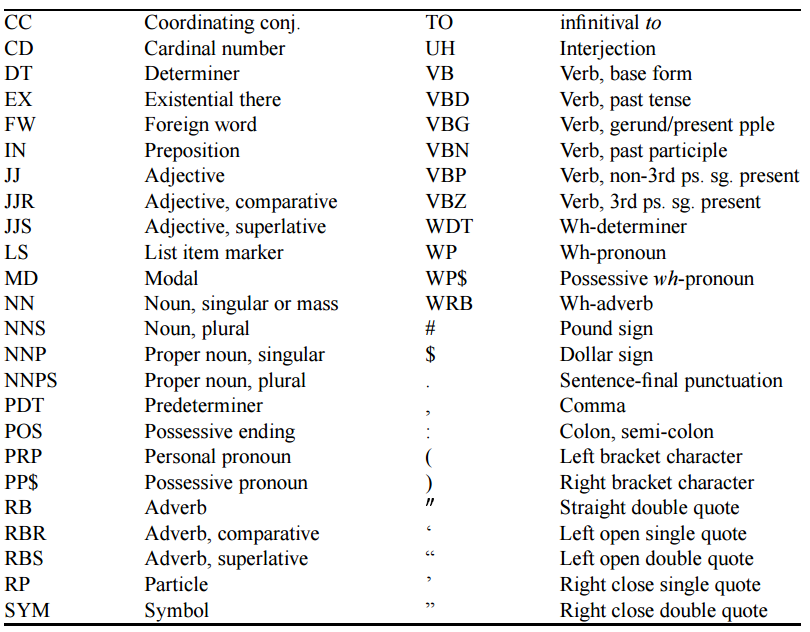
\includegraphics[width=12.823cm,height=8.004cm]{graficos/fuentes/WordTags.png}
  \caption{POS tags de Penn Treebank}
  \label{fig:word-tags}
\end{figure}


\begin{figure}[H]
  \centering
    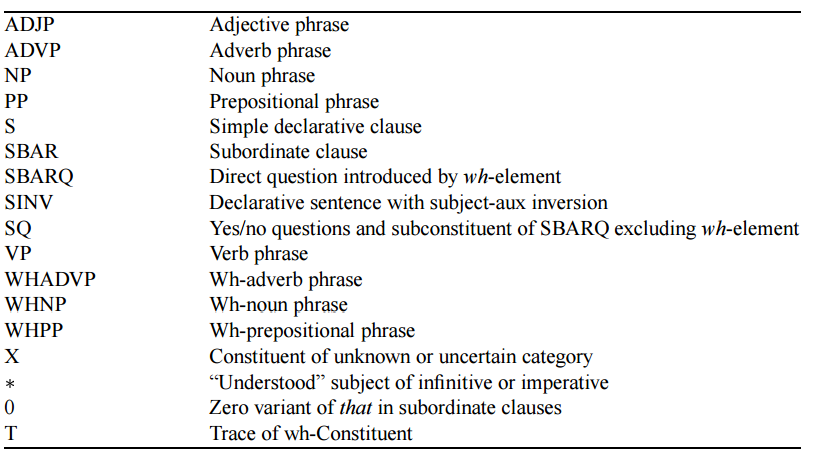
\includegraphics[width=12.823cm,height=8.004cm]{graficos/fuentes/SyntaxTags.png}
  \caption{Conjunto de tags para nodos intermedios del árbol sintáctico}
  \label{fig:syntax-tags}
\end{figure}


Las reglas que construimos son las siguientes (notar que los nombres pueden denotar una direccionalidad, pero las relaciones son simétricas.
Utilizamos NNx para denotar cualquier hoja sustantivo, adjetivo o adverbio (JJ, JJR, JJS, NN, NNS, NNP, NNPS, RB, RBR, RBS, CD), NN para denotar estrictamente sustantivos (NN, NNS, NNP, NNPS) y Nx para denotar cualquier sintagma relacionado a estos tipos de hojas (nodos intermedios): (ADJP, ADVP, NP, S)

%TODO: hacer esto lindo
\begin{enumerate}
\item Hermanos:
  \begin{itemize}
    \item  NNx $\Leftrightarrow$ NNx $\Leftrightarrow$ Wx si comparten el mismo el mismo padre
  \end{itemize}
\item Qwords a sustantivo:
  \begin{itemize}
    \item Una Wx dentro de un WHNP $\Rightarrow$ un NN dentro de uno o más Nx dentro de un VP dentro de un SQ con el mismo SBARQ como padre.
  \end{itemize}
\item Sintagma nominal a sintagma preposicional:
  \begin{itemize}
    \item NN dentro de un Nx $\Rightarrow$ NNx dentro de uno o más Nx dentro de un PP con el mismo padre que el NP original
  \end{itemize}
\item Sintagma nominal a sintagma verbal
    \begin{itemize}
      \item NN dentro de un Nx $\Rightarrow$ NNx dentro de uno o más Nx dentro de un VP del mismo padre que el NP original
    \end{itemize}
\item Sintagma preposicional a sintagma preposicional:
  \begin{itemize}
    \item NNx dentro de un PP $\Rightarrow$ NNx dentro de uno o más Nx dentro de un PP con el mismo padre que el NP original
  \end{itemize}
  \item Términos a tokens:
  \begin{itemize}
    \item Dos tokens están asociados si cualquier término de uno está asociado a cualquier término de otro.
  \end{itemize}
\end{enumerate}

En los ejemplos presentados, los pares de términos asociados según estas reglas son los siguientes. Para el primero, (hp, jobs), (unix, system)  (regla 1), (what, hp), (what, jobs) (regla 2) y, finalmente, (hp, unix), (hp, system), (job, unix), (jobs, system) (regla 3). Para el segundo, (us, states) (regla 1), (what, capitals) (regla 2) y (capitals, us) y (capitals, states) (regla 3). Para el tercero, (what, names) (regla 2), (names, cities) y (cities, argentina) (regla 3).
\newline

La definición de las reglas se hizo a prueba y error y es posible que sea simple, para alguien con mayores conocimientos lingüísticos, mejorarlas. Probablemente tenga sentido diferenciar entre sustantivos principal y modificador (Unix y system, por ejemplo) y modificar las reglas 3 y 4 para conectar solo los principales, entre otras mejoras. El sistema ofrece también la opción de no evaluar las asociaciones sintácticas en absoluto, en cuyo caso se mejora la performance pero aparecen nuevas traducciones válidas que podrían haber sido filtradas por estas condiciones, que el usuario deberá desambiguar manualmente).
Además, estas reglas seguramente sean insuficientes y estén dejando afuera varias preguntas que deberían poder procesarse.

Finalmente, todos los resultados de max-flow que cumplen con las condiciones de 1 a  4 son traducciones válidas, que pasan al MappingFilter, que realiza ciertos filtrados que describiremos, de nuevo, en un título aparte.

El resultado de este módulo es una lista de Mappings (una estructura que contiene 1) una tokenización completa de la pregunta original y 2) un mapeo válido entre cada token de la misma en un elemento de la base de datos). Cada mapeo es una traducción válida de la pregunta. Si existe solo uno, entonces este mapeo se traducirá en una query que generará el resultado. Si no, corresponde al MappingFilter realizar filtrados inteligentes de las múltiples soluciones y, en caso de que continuen existiendo múltiples soluciones, entonces se consultará al usuario qué quiso preguntar. Por otro lado, si no fue posible generar ninguna traducción válida, se retornará al usuario sin respuesta, pidiéndole que vuelva a escribir su pregunta de otro modo.

\subsubsection*{MappingFilter}
\label{subsubsec:mapping-filter}

La clase $uba.app.MappingFilter$ es responsable, en primer lugar, de quitar las traducciones válidas repetidas y, en segundo lugar, de aplicar una serie de reglas también de filtrado. Para eliminar las traducciones repetidas, las transformamos en queries y simplemente comparamos por igualdad, ya que el generador de queries ordena las cláusulas generando, para inputs iguales pero diferentemente ordenados, la misma query.
Además de este filtro, aplicamos tres reglas más, de creación propia. En primer lugar, eliminamos ``semi duplicados'', que consisten en atributos similares en la base de datos, en concreto, para esta base de datos, consideramos semi-duplicada a una query que consulta por Country.Name y por Country.LocalName solamente. La segunda y la tercera regla, están basadas en la misma idea: en el caso en que exista más de una traducción válida en la cual la qword esté asociada con un atributo \textit{implícito}, por como está el sistema definido, también estará asociado con todos los atributos que pueda estarlo (ver tabla \allref{table:atributos-qwords} para las compatibilidades definidas). Esto implica que, por ejemplo, para cualquier pregunta cuya qword sea 'what' y no tenga su atributo asociado explícito, habrá 16 diferentes traducciones válidas. En los trabajos sobre los que basamos nuestro proyecto este problema no está mencionado y en los ejemplos presentados no es visible. Lo que hicimos en este caso es aplicar dos conceptos de preferencia. La segunda regla, prefiere, entre los atributos implícitos posibles, aquellos cuya relación está mencionada en la pregunta (si hubiera alguna). La tercer regla, señala un orden de preferencia entre los atributos mismos, una vez especificada la relación. El atributo implicito preferido está marcado en negrita en la tabla \ref{table:atributos-qwords}. Si tras aplicar estar reglas siguen existiendo más de una traducción válida, entonces damos al usuario el control, pidiendo por una desambiguación.


\subsubsection*{QueryGenerator}
\label{subsubsec:query-generator}

El procedimiento para generar una query a partir de una traducción válida es exactamente el mismo que se desarrollo en \ref{subsec:closed-domain} y está implementado en el método Mapping.query().


\subsubsection*{MainProcessor}
\label{subsubsec:main-processor}

Finalmente, el punto de entrada de todo el sistema es $uba.app.MainProcessor$, que puede utilizarse especificando el parámetro -q QUESTION en cuyo caso responderá a esa pregunta y retornará el control o bien sin parámetros, en cuyo caso ingresa en un loop de preguntas-respuestas. El resultado para cada pregunta es cero, una o más queries de SQL.
Agregamos la opción de desambiguación para que el usuario elija entre dos o más queries si no se pudo generar una y también una presentación de las respuestas una vez determinada la query final, pero es más bien experimental y poco sólido.

\subsection{Ejemplos}
\label{subsec:popescu-ejemplos}

\subsubsection*{Ejemplo 1: ``Who is the head of state of Zimbabwe?''}

Consideremos nuestro primer ejemplo, una corrida trivial: ``Who is the head of state of Zimbabwe?''.

El primer paso es el tokenizer que, según expusimos, consta de los siguientes 7 pasos:

\begin{enumerate}
  \item Separar la pregunta en palabras, eliminar puntuaciones y pasar a lower case:
  \begin{itemize}
    \item \{who, is, the, head, of, state, of, zimbabwe\}
  \end{itemize}
  \item Lematizar las palabras:
  \begin{itemize}
    \item Todas las palabras ya están en su forma lematizada
  \end{itemize}
  \item Eliminar marcadores sintácticos:
  \begin{itemize}
    \item \{who, head, state, zimbabwe\}
  \end{itemize}
  \item Obtener tokens para cada lema ($Lexicon.getTokens()$)
  \begin{itemize}
    \item $getTokens(who)\ \rightarrow \{$'who'$\}$
    \item $getTokens(head)\ \rightarrow \{$ 'head country', 'head teacher body politic', 'head body politic', 'head teacher land', 'read / write head dos', 'heading provincial', 'heading state', 'heading commonwealth', 'head teacher dos', 'head teacher country', 'read / write head body politic', 'head word land', 'head state of matter', 'read / write head provincial', 'read / write head state department', 'read / write head department of state', 'head province', 'heading body politic', 'heading res publica', 'read / write head nation', (51 más)...$\}$

    \item $getTokens(state)\ \rightarrow  \{$'heart eastern united states', 'centre eastern united states', 'central eastern united states', 'centrical eastern united states', 'midsection eastern united states', 'midriff eastern united states', 'centric eastern united states', 'center eastern united states', 'middle eastern united states', 'eye eastern united states', 'camellia state yaman', 'frederick north western united states', 'compass north western united states', 'north western united states', 'second earl of guilford western united states', 'magnetic north western united states', 'northward western united states', 'due north western united states', 'union western united states', (702 más)...$\}$
    \item $getTokens(zimbabwe)\ \rightarrow \{$'zimbabwe', 'republic of zimbabwe', 'capital of zimbabwe'$\}$
  \end{itemize}
  \item Para cada token potencial (resultado del paso anterior) verificar que todos sus lemas están presentes en el conjunto de lemas de la pregunta original.
  \begin{itemize}
    \item $getTokens(who)\ \rightarrow \{$'who'$\}$
    \item $getTokens(head)\ \rightarrow \{$'head state', 'heading state', 'head of state' $\}$
    \item $getTokens(state)\ \rightarrow  \{$  'state', 'head state', 'heading state', 'head of state'$\}$
    \item $getTokens(zimbabwe)\ \rightarrow \{$'zimbabwe'$\}$
  \end{itemize}
  \item Generar el conjunto de partes de todos los tokens hasta aquí obtenidos.
  \newline
  \{ $\emptyset$, \{'head of state', 'zimbabwe'\}, \{'zimbabwe', 'state'\}, \{'zimbabwe', 'heading state', 'state', 'head state', 'who'\}, \{'head of state', 'zimbabwe', 'who'\}, \{'head of state', 'zimbabwe', 'heading state', 'head state', 'who'\}, \{'head of state', 'zimbabwe', 'heading state', 'who'\}, \{'head of state', 'zimbabwe', 'heading state', 'state'\}, \{'head of state', 'zimbabwe', 'heading state', 'state', 'who'\}, \{'who'\}, \{'head of state', 'heading state', 'head state'\}, \{'head of state'\}, \{'state', 'who'\}, \{'head of state', 'zimbabwe', 'heading state', 'head state'\}, \{'heading state', 'state', 'who'\}, \{'heading state', 'state'\}, \{'heading state', 'who'\}, \{'head of state', 'who'\}, \{'head of state', 'zimbabwe', 'state', 'who'\}, \{'head of state', 'state', 'head state'\}, \{'zimbabwe', 'heading state', 'state', 'who'\}, \{'zimbabwe', 'head state', 'who'\}, \{'zimbabwe', 'heading state', 'who'\}, \{'head of state', 'heading state', 'who'\}, \{'state', 'head state', 'who'\}, \{'head state'\}, \{'heading state', 'state', 'head state'\}, \{'head of state', 'state', 'who'\}, \{'zimbabwe'\}, \{'state', 'head state'\}, \{'state'\}, \{'head of state', 'heading state', 'state'\}, \{'zimbabwe', 'state', 'who'\}, \{'zimbabwe', 'state', 'head state'\}, \{'head of state', 'zimbabwe', 'heading state', 'state', 'head state'\}, \{'head of state', 'zimbabwe', 'heading state', 'state', 'head state', 'who'\}, \{'head of state', 'zimbabwe', 'state', 'head state', 'who'\}, \{'heading state', 'head state', 'who'\}, \{'heading state'\}, \{'head of state', 'zimbabwe', 'state'\}, \{'head of state', 'zimbabwe', 'head state', 'who'\}, \{'head of state', 'heading state', 'state', 'who'\}, \{'head of state', 'zimbabwe', 'state', 'head state'\}, \{'head of state', 'zimbabwe', 'heading state'\}, \{'head of state', 'zimbabwe', 'head state'\}, \{'head of state', 'heading state', 'state', 'head state'\}, \{'head state', 'who'\}, \{'head of state', 'state'\}, \{'head of state', 'heading state', 'head state', 'who'\}, \{'head of state', 'heading state', 'state', 'head state', 'who'\}, \{'zimbabwe', 'heading state'\}, \{'head of state', 'head state'\}, \{'heading state', 'state', 'head state', 'who'\}, \{'zimbabwe', 'state', 'head state', 'who'\}, \{'heading state', 'head state'\}, \{'head of state', 'head state', 'who'\}, \{'head of state', 'heading state'\}, \{'zimbabwe', 'heading state', 'state'\}, \{'zimbabwe', 'heading state', 'head state', 'who'\}, \{'zimbabwe', 'who'\}, \{'zimbabwe', 'head state'\}, \{'zimbabwe', 'heading state', 'head state'\}, \{'zimbabwe', 'heading state', 'state', 'head state'\}, \{'head of state', 'state', 'head state', 'who'\} \}
  \item Para cada uno de estos subconjuntos, verificar 1) que los lemas de sus tokens cubran completamente
los lemas significativos de la pregunta original y 2) que no haya lemas repetidos
entre los tokens.
  \begin{itemize}
    \item Los lemas significativos son los obtenidos en el bullet 4: \{who, head, state, zimbabwe\}
    \item Las tokenizaciones que los cubren sin repetir lemas son: \{'who', 'head state', 'zimbabwe'\},
    \{'who', 'heading state', 'zimbabwe'\} y  \{'who', 'head of state', 'zimbabwe'\}, con lo que queda eliminado el token 'state' y las repeticiones de los tokens que refieren tanto a 'head' como a 'state', quedando solo las diferentes formulaciones sinónimas del mismo elemento de la base de datos.
  \end{itemize}
\end{enumerate}

Es decir, el Tokenizer encontró tres conjuntos de tokens completos para la pregunta, Tokenizer.generateCompleteTokenizations(``Who is the head of state of Zimbabwe?'') $\rightarrow$ [\{ `who', `head state', `zimbabwe'\}, \{`who', `heading state', `zimbabwe'\}, \{`who', `head of state', `zimbabwe'\}].

El siguiente paso es el Matcher, que construye el grafo de atributos y valores para cada uno de las tokenizaciones completas y decide si existe un conjunto de elementos de la base de datos que permita establecer la traducción. Presentamos aquí solamente el grafo para la primer tokenización completa, que puede verse en la figura \ref{grafo-1}. Las otras tokenizaciones tienen un grafo análogo y generaran el mismo resultado, que será filtrado luego por el EquivalenceChecker. Notar que no es esta repetición de tokenizaciones lo que filtra el Matcher, sino la ambigüedad introducida por un token que puede referir a dos o más elementos de la base de datos (este problema no ocurre en este primer ejemplo).
 Para construirlo, primero, se consulta al Lexicón por el tipo y los elementos asociados de cada token mediante el servicio $getMatchingElements$ como se puede ver en la tabla \ref{table:get-matching-elements-1}.
\begin{center}
\begin{table}[h]
\centering
\begin{tabular}{| p{3cm} | l | l | p{6cm} |}
\hline
Token & Tipos & Elementos & Detalle \\ \hline
zimbabwe & Value & Zimbabwe & Valor del Atributo Name de la tabla Country\\ \hline
head state, head of state, heading state & Attribute & HeadOfState & Atributo de la tabla Country\\ \hline
who & WhValue/Value & Who & Q-valor compatible con: Atributo HeadOfState de la tabla Country\\ \hline
\end{tabular}
\caption{Resultados de $getMatchingElements$ para ``Who is the head of state of Zimbabwe?''}
\label{table:get-matching-elements-1}
\end{table}
\end{center}

En este primer ejemplo el grafo no desambigua ninguna relación token-elemento ya que no hay ningún token con más de un elemento asociado, por lo que el grafo de max-flow no tiene ningun atractivo especial y es construido siguendo el procedimiento reseñado en \ref{subsec:closed-domain} Al ejecutar el algoritmo de max-flow sobre el grafo, se obtiene que el flujo máximo es 2 y los pares (Who, Country.HeadOfState), (Country.Name, Zimbabwe), sin generar ningún otro flujo alternativo como se ve en la figura \ref{grafo-1}.



\begin{figure}
\hspace*{-1.2cm}
\centering
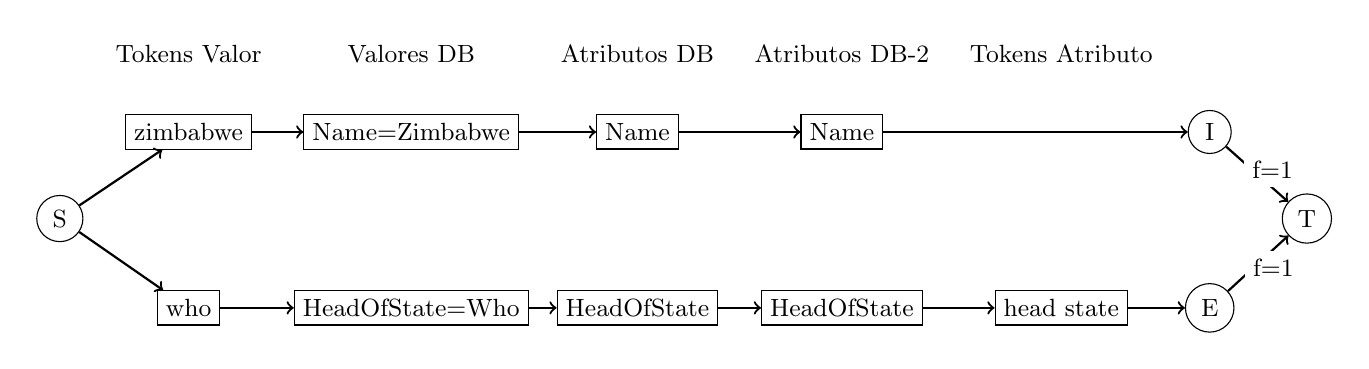
\begin{tikzpicture}
\small
\matrix [column sep=3mm, row sep=5mm] {
   & \node (title1) [] {Tokens Valor};
   & \node (title) [] {Valores DB};
   & \node (title) [] {Atributos DB};
   & \node (title) [] {Atributos DB-2};
   & \node (title) [] {Tokens Atributo};& &

  \\
     &  \node (token_zimbabwe) [draw, shape=rectangle] {zimbabwe}; & \node (value_zimbabwe) [draw, shape=rectangle] {Name=Zimbabwe}; & \node (attr_name_1) [draw, shape=rectangle] {Name}; &  \node (attr_name_2) [draw, shape=rectangle] {Name};& & \node (i) [draw, shape=circle] {I}; &

  \\
  \node (source) [draw, shape=circle] {S}; & & & & & & & &\node (sink) [draw, shape=circle] {T};
  \\
   &  \node (token_who) [draw, shape=rectangle] {who}; & \node (value_who) [draw, shape=rectangle] {HeadOfState=Who}; & \node (attr_head_1) [draw, shape=rectangle] {HeadOfState}; &  \node (attr_head_2) [draw, shape=rectangle] {HeadOfState};&
   \node (token_head) [draw, shape=rectangle] {head state}; &
   \node (e) [draw, shape=circle] {E}; &

   \\
};
\draw[->, thick] (source) -- (token_zimbabwe);
\draw[->, thick] (token_zimbabwe) -- (value_zimbabwe);
\draw[->, thick] (value_zimbabwe) -- (attr_name_1);
\draw[->, thick] (attr_name_1) -- (attr_name_2);
\draw[->, thick] (attr_name_2) -- (i);
\draw[->, thick] (source) -- (token_who);
\draw[->, thick] (token_who) -- (value_who);
\draw[->, thick] (value_who) -- (attr_head_1);
\draw[->, thick] (attr_head_1) -- (attr_head_2);
\draw[->, thick] (attr_head_2) -- (token_head);
\draw[->, thick] (token_head) -- (e);

\draw[->, thick] (i) -- (sink) node [near end, fill=white, above] {f=1};
\draw[->, thick] (e) -- (sink) node [near end, fill=white, below] {f=1};
\end{tikzpicture}
\caption{Grafo de atributo-valor para la primer tokenización completa de ``Who is the head of state of Zimbabwe?''}
\label{grafo-1}
\end{figure}

El próximo paso es evaluar que los términos del par de tokens (`who', `head state') estén sintácticamente asociados en el
parse tree generado por el algoritmo de Charniak según nuestras reglas. El arbol sintáctico para la pregunta es el siguiente:

\begin{center}[h]
\Tree [.S1 [.SBARQ [.WHNP [.WP \textbf{Who} ] ] [.SQ [.VP [.AUX is ] [.NP [.NP [.DT the ] [.NN \textbf{head} ] ] [.PP [.IN of ] [.NP [.NN state ] ] ] [.PP [.IN of ] [.NP [.NNP Zimbabwe ] ] ] ] ] ] [.. ? ] ] ] \\
``Who is the head of state of Zimbabwe?''
\end{center}

La regla 2 (q-word a sustantivo) vincula los términos 'who' con 'head', mientras que la 6 (términos a tokens), asocia los tokens 'who' con 'head state', cumpliendo las condiciones sintácticas requeridas por la definición de traducción válida. Por su parte, el atributo Name es implícito, lo que significa que no posee ningún token asociado y, por lo tanto, no debe cumplir la regla de traducciones válidas. Además, como no hay ninguna relación mencionada explicitamente, los tokens cubren todos los términos significativos de la pregunta y no hay ningún término repetido entre los tokens, esto significa que tenemos una (única) traducción válida para esta tokenización completa, constando de los siguiente elementos de la base de datos apareados: (Atributo Country.Name, Valor Country.Name$=$Zimbabwe), (Atributo Country.HeadOfState, Q-Valor Who).

Las otras dos tokenizaciones generan la misma traducción y sus repeticiones son eliminadas por el $EquivalenceChecker$.
Finalmente, esta única traducción pasa al $QueryGenerator$ que la traduce univocamente en una query, aplicando las reglas descriptas en \ref{subsec:closed-domain}:

``\textbf{SELECT} Country.HeadOfState \textbf{FROM} Country \textbf{WHERE} Country.Name$=$`Zimbabwe' '', cuyo resultado es ``Robert G. Mugabe''.

\subsubsection*{Ejemplo 2: ``What caribbean countries are also considered north american?''}

Consideremos nuestro segundo ejemplo: ``What caribbean countries are also considered north american?''.

El primer paso es el tokenizer que, según expusimos, consta de los siguientes 7 pasos:

\begin{enumerate}
  \item Separar la pregunta en palabras, eliminar puntuaciones y pasar a lower case:
  \begin{itemize}
    \item \{what, caribbean, countries, are, also, considered, north, american\}
  \end{itemize}
  \item Lematizar las palabras:
  \begin{itemize}
    \item \{what, caribbean, country, is, also, consider, north, american\}
  \end{itemize}
  \item Eliminar marcadores sintácticos:
  \begin{itemize}
    \item \{what, caribbean, country, north, american\}
  \end{itemize}
  \item Obtener tokens para cada lema ($Lexicon.getTokens()$)
  \begin{itemize}
    \item $getTokens(what)\ \rightarrow \{$'what'$\}$
    \item $getTokens(caribbean)\ \rightarrow \{$'caribbean sea', 'caribbean', 'micronesia caribbean sea', 'federated states of micronesia caribbean', 'tt caribbean sea', 'micronesia / caribbean', 'tt caribbean', 'micronesia caribbean', 'federated states of micronesia caribbean sea'$\}$
    \item $getTokens(country)\ \rightarrow  \{$'country codification', 'country computer code', 'country codify', 'country code', 'baltic country', 'baltic language country', 'baltic sea country', 'north germanic language country', 'norse country', 'nordic country', 'scandinavian country', 'scandinavian language country', 'north germanic country', 'independent christian church country', 'free lance christian church country', 'self - employed person church building country', 'freelance church country', 'independent church service country', 'freelancer churchly country', 'free - lance churchly country', (149 más)...$\}$
    \item $getTokens(north)\ \rightarrow \{$'jabir aluminum ahmad aluminum jabir heart of dixie north borneo', 'jabir alabama ahmad camellia state jabir aluminum north borneo', 'jabir aluminize ahmad aluminise jabir aluminous north borneo', 'jabir aluminium ahmad camellia state jabir aluminize north borneo', 'jabir aluminize ahmad camellia state jabir aluminise north borneo', 'jabir al ahmad al jabir aluminium north borneo', 'jabir aluminous ahmad al jabir aluminise north borneo', 'jabir heart of dixie ahmad aluminous jabir camellia state north borneo', 'jabir aluminous ahmad camellia state jabir aluminous north borneo', 'jabir aluminium ahmad al jabir aluminize north borneo', 'jabir al ahmad aluminize jabir alabama north borneo', 'jabir aluminous ahmad al jabir heart of dixie north borneo', 'jabir aluminum ahmad aluminous jabir aluminum north borneo', 'jabir aluminum ahmad alabama jabir al north borneo', 'jabir heart of dixie ahmad aluminise jabir aluminous north borneo', 'jabir atomic number 13 ahmad aluminum jabir atomic number 13 north borneo', 'jabir aluminise ahmad alabama jabir aluminum north borneo', 'jabir aluminum ahmad aluminize jabir aluminize north borneo', 'jabir aluminium ahmad al jabir aluminous north borneo', 'jabir aluminous ahmad aluminium jabir camellia state north borneo', (2237 más)...$\}$
    \item $getTokens(american)\ \rightarrow \{$ 'american virgin islands', 'southward american', 'south american', 'due south american', 's american', 'dixieland american', 'dixie american', 'confederate states of america american', 'confederacy american', 'confederate states american', 'northward american', 'due north american', 'frederick north american', 'n american', 'second earl of guilford american', 'union american', 'north american', 'compass north american', 'magnetic north american', 'american - indian language spoken language', (169 más)...$\}$
  \end{itemize}
  \item Para cada token potencial (resultado del paso anterior) verificar que todos sus lemas están presentes en el conjunto de lemas de la pregunta original.
  \begin{itemize}
    \item $getTokens(what)\ \rightarrow \{$'what'$\}$
    \item $getTokens(caribbean)\ \rightarrow \{$'caribbean'$\}$
    \item $getTokens(country)\ \rightarrow  \{$'country'$\}$
    \item $getTokens(north)\ \rightarrow \{$'north american'$\}$
    \item $getTokens(american)\ \rightarrow \{$'north american', 'american'$\}$
  \end{itemize}
  \item Generar el conjunto de partes de todos los tokens hasta aquí obtenidos.
  \newline
   \{ $\emptyset$, \{'north american'\}, \{'what', 'american', 'country'\}, \{'north american', 'what', 'american', 'country'\}, \{'american', 'caribbean'\}, \{'north american', 'what', 'american'\}, \{'what', 'country'\}, \{'north american', 'what', 'american', 'caribbean', 'country'\}, \{'caribbean'\}, \{'north american', 'what', 'caribbean'\}, \{'north american', 'american', 'country'\}, \{'north american', 'what'\}, \{'american'\}, \{'north american', 'american', 'caribbean', 'country'\}, \{'north american', 'what', 'caribbean', 'country'\}, \{'american', 'country'\}, \{'what', 'american', 'caribbean', 'country'\}, \{'north american', 'country'\}, \{'what', 'american'\}, \{'what', 'caribbean', 'country'\}, \{'american', 'caribbean', 'country'\}, \{'north american', 'caribbean'\}, \{'country'\}, \{'north american', 'what', 'american', 'caribbean'\}, \{'north american', 'caribbean', 'country'\}, \{'north american', 'what', 'country'\}, \{'what', 'caribbean'\}, \{'north american', 'american', 'caribbean'\}, \{'what'\}, \{'north american', 'american'\}, \{'what', 'american', 'caribbean'\}, \{'caribbean', 'country'\}\}
  \item Para cada uno de estos subconjuntos, verificar 1) que los lemas de sus tokens cubran completamente
los lemas significativos de la pregunta original y 2) que no haya lemas repetidos
entre los tokens.
  \begin{itemize}
    \item Los lemas significativos son los obtenidos en el bullet 4: \{what, caribbean, country, north, american\}
    \item Solo una tokenización los cubren sin repetir lemas: \{'north american', 'what', 'caribbean', 'country'\}, con lo que queda eliminado el token 'american'.
  \end{itemize}
\end{enumerate}

Es decir, el Tokenizer encontró un conjunto de tokens completo para la pregunta, Tokenizer.generateCompleteTokenizations(``What caribbean countries are also considered north american?'') $\rightarrow$ [ \{what, caribbean, country, north american\}].

El siguiente paso es el grafo del Matcher, que en este caso sí desambigua un token de valor. Como puede verse en \ref{table:get-matching-elements-2}, al token 'caribbean' le corresponden dos posibles valores: valor del atributo Region de la tabla Country y también valor del atributo Continent de la tabla Country.

En este ejemplo el grafo decide entre dos interpretaciones posibles  (Ver grafo \ref{grafo-2}) para el token 'caribbean', que puede ser un valor tanto del atributo Region como del atributo Continent. Teniendo presente el token 'north american', que solo puede tomar el atributo Continent, para maximizar el flujo el algoritmo asigna 'caribean' a Region, obteniendo un flujo de 3, que es el máximo y eliminando así la posibilidad de relacionar este token de valor con el atributo Continent.


%TODO: entender porque tuve que limitar el tipado por elemento (atributo > valor y relacion > valor).
\begin{center}
\begin{table}[h]
\centering
\begin{tabular}{| p{2cm} | p{2cm} | p{2cm} | p{6cm} |}
\hline
Token & Tipos & Elementos & Detalle \\ \hline
caribbean & Value & North America & Valor de los Atributo Region y Continent de la tabla Country\\ \hline
north american & Value & Caribbean & Valor del Atributo Region de la tabla Country\\ \hline
country & Relation & Country & Relación Country\\ \hline
what & WhValue / Value & What & Q-valor compatible con: Atributos GovernmentForm, Population, GNP, Name, Capital, LocalName, Continent, Region, Code, LifeExpectancy y SurfaceArea de la tabla Country, District, Population y Name de la tabla City e ISOfficial y Percentage de la tabla Language\\ \hline
\end{tabular}
\caption{Resultados de $getMatchingElements$ para ``What caribbean countries are also considered north american?''}
\label{table:get-matching-elements-2}
\end{table}
\end{center}

\begin{figure}
\hspace*{-1.5cm}
\centering
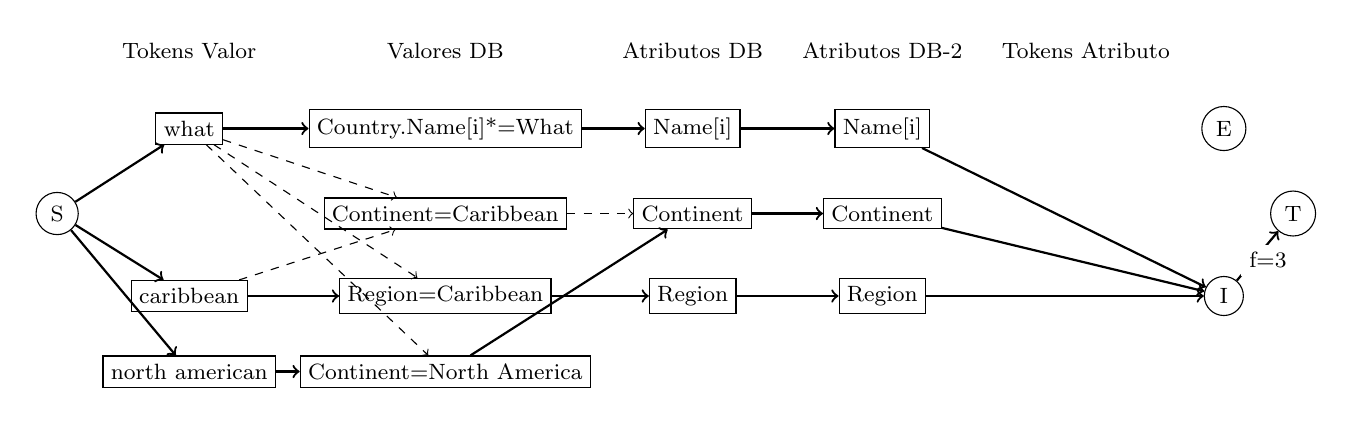
\begin{tikzpicture}
\footnotesize
\matrix [column sep=3mm, row sep=5mm] {
   & \node (title1) [] {Tokens Valor};
   & \node (title) [] {Valores DB};
   & \node (title) [] {Atributos DB};
   & \node (title) [] {Atributos DB-2};
   & \node (title) [] {Tokens Atributo};& & \\

   &  \node (token_what) [draw, shape=rectangle] {what}; & \node (value_what) [draw, shape=rectangle] {Country.Name[i]*=What}; & \node (attr_name_1) [draw, shape=rectangle] {Name[i]}; &  \node (attr_name_2) [draw, shape=rectangle] {Name[i]}; & & \node (e) [draw, shape=circle] {E};  & \\

   \node (source) [draw, shape=circle] {S}; & & \node (value_caribbean_2) [draw, shape=rectangle] {Continent=Caribbean}; & \node (attr_continent_1) [draw, shape=rectangle] {Continent}; &  \node (attr_continent_2) [draw, shape=rectangle] {Continent}; & & &\node (sink) [draw, shape=circle] {T}; \\

   & \node (token_caribbean) [draw, shape=rectangle] {caribbean};
   & \node (value_caribbean) [draw, shape=rectangle] {Region=Caribbean};
   & \node (attr_region_1) [draw, shape=rectangle] {Region};
   & \node (attr_region_2) [draw, shape=rectangle] {Region};
   & & \node (i) [draw, shape=circle] {I}; & \\


   & \node (token_north) [draw, shape=rectangle] {north american}; & \node (value_north) [draw, shape=rectangle] {Continent=North America}; &  & & & & \\
};

\draw[->, thick] (source) -- (token_caribbean);
\draw[->, thick] (token_caribbean) -- (value_caribbean);
\draw[->, thick] (value_caribbean) -- (attr_region_1);
\draw[->, thick] (attr_region_1) -- (attr_region_2);
\draw[->, thick] (attr_region_2) -- (i);

\draw[->, dashed] (token_caribbean) -- (value_caribbean_2);
\draw[->, dashed] (value_caribbean_2) -- (attr_continent_1);
\draw[->, thick] (attr_continent_1) -- (attr_continent_2);
\draw[->, thick] (attr_continent_2) -- (i);

\draw[->, thick] (source) -- (token_north);
\draw[->, thick] (token_north) -- (value_north);
\draw[->, thick] (value_north) -- (attr_continent_1);


\draw[->, thick] (source) -- (token_what);
\draw[->, thick] (token_what) -- (value_what);
\draw[->, dashed] (token_what) -- (value_caribbean);
\draw[->, dashed] (token_what) -- (value_caribbean_2);
\draw[->, dashed] (token_what) -- (value_north);
\draw[->, thick] (value_what) -- (attr_name_1);
\draw[->, thick] (attr_name_1) -- (attr_name_2);
\draw[->, thick] (attr_name_2) -- (i);

\draw[->, thick] (i) -- (sink) node [near end, fill=white, below] {f=3};
\end{tikzpicture}
\caption{Grafo de atributo-valor para la primer tokenización completa de ``What caribbean countries are also considered north american?''}
\label{grafo-2}
\end{figure}


Como no hay tokens de atributo explícitos, solo queda verificar la regla relacionada con los tokens de relación: Country es compatible con todos los tokens de valor que aparecen en la pregunta y, en particular, está sintácticamente asociada a what (regla 2), por lo que las condiciones de traducción válida se cumplen.

Esto nos da una única traducción válida, pero en realidad el $Matcher$ genera 16, una por cada atributo implícito posible compatible con la q-word 'What'. Notar que Country.Name no tiene ninguna particularidad especial, al menos no para el $Matcher$, sobre las demás posibilidades listadas en \ref{table:get-matching-elements-2}. Pero de esto se ocupa el $MappingFilter$ con las tres reglas especiales que agregamos. Dado que la relación $country$ está presente en la pregunta y no así las otras dos, aplicando las reglas de preferencia de atributos implícitos nos quedamos solo con la asociación Country.Name$=$What.

\begin{center}
\Tree
[.S1 [.SBARQ [.WHNP [.WP What ] ] [.SQ [.NP [.JJ caribbean ] [.NNS countries ] ] [.VP [.AUX are ] [.ADVP [.RB also ] ] [.VP [.VBN considered ] [.S [.ADJP [.JJ north ] [.JJ american ] ] ] ] ] ] [.. ? ] ] ]
 \\
Charniak parse tree para ``What caribbean countries are also considered north american?''
\end{center}

Esta única traducción pasa al $QueryGenerator$ que la traduce univocamente en una query, aplicando las reglas descriptas en \ref{subsec:closed-domain}:
``\textbf{SELECT DISTINCT} Country.Name \textbf{FROM} Country \textbf{WHERE} Country.Continent $=$ 'North America' \textbf{AND} Country.Region $=$ 'Caribbean''' cuyo resultado es la siguiente lista:

\begin{itemize}
 \item Aruba
 \item Anguilla
 \item Netherlands Antilles
 \item Antigua and Barbuda
 \item Bahamas
 \item Barbados
 \item Cuba
 \item Cayman Islands
 \item Dominica
 \item Dominican Republic
 \item Guadeloupe
 \item Grenada
 \item Haiti
 \item Jamaica
 \item Saint Kitts and Nevis
 \item Saint Lucia
 \item Montserrat
 \item Martinique
 \item Puerto Rico
 \item Turks and Caicos Islands
 \item Trinidad and Tobago
 \item Saint Vincent and the Grenadines
 \item Virgin Islands, British
 \item Virgin Islands, U.S.
\end{itemize}


\subsection{Conclusiones, limitaciones y trabajo futuro}
\label{subsec:popescu-cierre}

Las diferentes limitaciones y mejoras de nuestra implementación actual fueron mencionadas durantes la exposición de la misma que realizamos a lo largo de este capítulo: esta sección las presenta juntas para facilitar el acceso.

En un nivel técnico, habría una enorme mejora de performance implementando el lexicón sobre una base de datos relacional. Los archivos json sirven para un modelo de escala pequeña, pero no permiten escalar ya que genera un tiempo de carga innecesario, así como también uso de memoria. Existen también una serie de clases con datos dentro del código que deberían separar archivos de configuración de códigos. Estas son TokenAugmenter, WhGenerator y Config. Estas clases requieren editar el código para aplicarlo sobre una nueva base de datos, cuando en realidad solo es necesario editar definiciones.

Más allá de estas mejoras técnicas, las siguientes mejoras permitirían incrementar la usabilidad y la eficacia del sistema:

\begin{itemize}
\item En el Lexicón, no generar sinónimos para nombres propios. Wordnet posee sinónimos para, por ejemplo \textit{Hugo} (Victor Hugo, etc) introduciendo ruido innecesario y fácilmente eliminable.
\item Lexicon: Desambiguador de sentidos para los sinónimos de los tokens. Este es un problema complejo de NLP e integrar una solución del mismo dentro del modelo ya definido podría redundar en un avance teórico. Desde un nivel más técnico y con mejor complejidad, también sería posible implementar un desambiguador supervisado.
\item Soportar desambiguación de relaciones en el Matcher.
\item Interfaz con el usuario: como mencionamos, el resultado es una query y la desambiguación es entre dos o más queries. Que el resultado sea una respuesta presentada en un formato amigable y que la desambiguación sea, también, presentada en un formato amigable es una mejora de usabilidad necesaria para utilizar el sistema en la vida real.
\item CharniakParseTree: evaluando con un lingüista profesional las reglas utilizadas para definir la \textit{asociación sintáctica} seguramente se obtengan reglas más eficaces.
\end{itemize}

Con esta lista terminamos la presentación de nuestro sistema closed domain en inglés. En el próximo capitulo daremos vuelta la página y presentaremos nuestro sistema open domain multilingüe.


%TODO: conclusiones